\documentclass[aspectratio=169,11pt]{beamer}

\usetheme{Madrid}
\usecolortheme{seahorse}
\useinnertheme{circles}
\setbeamertemplate{navigation symbols}{}
\setbeamertemplate{caption}{\raggedright\insertcaption\par}

\usepackage[T1]{fontenc}
\usepackage{amsmath,amssymb}
\usepackage{graphicx}
\usepackage{booktabs}
\usepackage{array}
\usepackage{xcolor}

\graphicspath{{../plots/}{../plots/fine/}}

% shorthands
\newcommand{\Cs}{$^{16}$C}
\newcommand{\Cse}{$^{17}$C}
\newcommand{\dpr}{(d,p)}
\newcommand{\dsdo}{$\mathrm{d}\sigma/\mathrm{d}\Omega$}
\newcommand{\chinu}{$\chi^2/\nu$}
\newcommand{\thcm}{$\theta_{\mathrm{c.m.}}$}
\newcommand{\Ex}{$E_x$}
\newcommand{\good}{\textcolor{green!55!black}{\textbf{\checkmark}}}
\newcommand{\warn}{\textcolor{orange!80!black}{\textbf{!}}}

\title[\Cs\dpr\Cse\ analysis]{Spectroscopy of unbound \Cse\ states\\ via \Cs\dpr\Cse\ at FRIB (a1975)}
\subtitle{Angular distributions, absolute normalization, and $L$ assignments}
\author[Y.~Ayyad]{Y.~Ayyad}
\institute[USC]{IGFAE -- Universidade de Santiago de Compostela}
\date{30 May 2026 \\ \footnotesize spectroscopic reference: Movilla \& Ayyad (2026-02)}

\begin{document}

{\setbeamertemplate{footline}{}
\begin{frame}\titlepage\end{frame}}

\begin{frame}{Outline}
  \tableofcontents
\end{frame}

% ======================================================================
\section{Reaction and method}

\begin{frame}{The experiment}
  \begin{columns}[T]
    \begin{column}{0.56\textwidth}
      \begin{itemize}
        \item \Cs\ beam in the AT-TPC, D$_2$ active target (FRIB exp.\ \textbf{a1975}).
        \item Beam energy: $188.33$ MeV total $=$ \textbf{11.77 MeV/u};
              $Q_{\mathrm{g.s.}}=-1.498$ MeV.
        \item Transfer populates \Cse\ states across the bound region and
              \textbf{seven unbound resonances}.
        \item Goal: per-state \dsdo\ on an \textbf{absolute scale} $\rightarrow$
              transferred-$L$ assignment by comparison with FRESCO ADWA shapes.
      \end{itemize}
      \vspace{0.4em}
      {\small Continuation of \texttt{C16dp\_fits}; data reduced with ATTPCROOT
      (\texttt{InterpSolver}).}
    \end{column}
    \begin{column}{0.44\textwidth}
      \small
      \centering
      \textbf{Unbound resonances fitted}\\[0.3em]
      \begin{tabular}{@{}ccc@{}}
        \toprule
        \Ex\,(MeV) & $J^\pi$ & $\Gamma$\,(keV)\\
        \midrule
        2.763 & $1/2^-$ & 50 \\
        2.980 & $3/2^+$ & 200 \\
        3.661 & \textit{new} & 398 \\
        4.231 & $3/2^+$ & 500 \\
        4.841 & $1/2^+$ & 300 \\
        5.91  & $3/2^+$ & 1500 \\
        6.30  & $5/2^+$ & 396 \\
        \bottomrule
      \end{tabular}
    \end{column}
  \end{columns}
\end{frame}

\begin{frame}{Analysis pipeline}
  \begin{enumerate}
    \item \textbf{Spectral fit} (\texttt{C16\_pd\_AngBins.C}): $Q$-corrected \Ex\
      spectrum, $12\times2.5^\circ$ bins ($10$--$40^\circ$).
      Inclusive fit pins BW positions/widths; per-bin fits free only amplitudes.
      \begin{itemize}\small
        \item 3 Gaussians (bound) $+$ 7 penetrability-modified Breit--Wigners
              $+$ 1n/2n phase space $+$ linear bg.
        \item energy-dependent $\Gamma$ via tabulated penetrabilities; analytic
              Voigt lineshape.
      \end{itemize}
    \item \textbf{Efficiency correction}: 8 \Ex-dependent tables, bilinear
      $(E_x,\theta)$ interpolation; $\varepsilon$-floor and $\varepsilon$-gradient cuts.
    \item \textbf{Absolute normalization} fixed by the \Cs(d,d) elastic channel.
    \item \textbf{$L$ scan}: each AD fit to FRESCO $L=0$--$3$ ADWA shapes; best $L$
      by \chinu.
    \item \textbf{Systematics}: 82-variant campaign $\rightarrow$ per-state envelope.
  \end{enumerate}
\end{frame}

% ======================================================================
\section{Spectral fit and bound states}

\begin{frame}{Inclusive \Ex\ spectrum: the global fit}
  \begin{columns}[T]
    \begin{column}{0.62\textwidth}
      \centering
      
\includegraphics[width=\linewidth]{plots_inclusive.png}
    \end{column}
    \begin{column}{0.38\textwidth}
      \small
      A localized $+2$--$4\sigma$ excess near $0.4$--$1.1$ MeV is not absorbed by
      the nominal model. Adding a \textbf{contaminant Gaussian} (centroid pegs at
      $\sim0.45$ MeV) restores an acceptable fit:
      \vspace{0.5em}
      \begin{tabular}{@{}lcc@{}}
        \toprule
        cuts & nominal & $+$contam\\
        \midrule
        loose  & 1.78 & \textbf{0.84}\\
        strict & 1.88 & \textbf{0.97}\\
        \bottomrule
      \end{tabular}
      \vspace{0.5em}\\
      Survives the strict cuts (centroid $0.450\!\to\!0.451$ MeV) $\Rightarrow$
      \textit{not} an AT-TPC edge artifact. Carried as a model-dependence
      systematic.
    \end{column}
  \end{columns}
\end{frame}

\begin{frame}{Bound states: angular distributions}
  \begin{columns}[T]
    \begin{column}{0.62\textwidth}
      \centering
      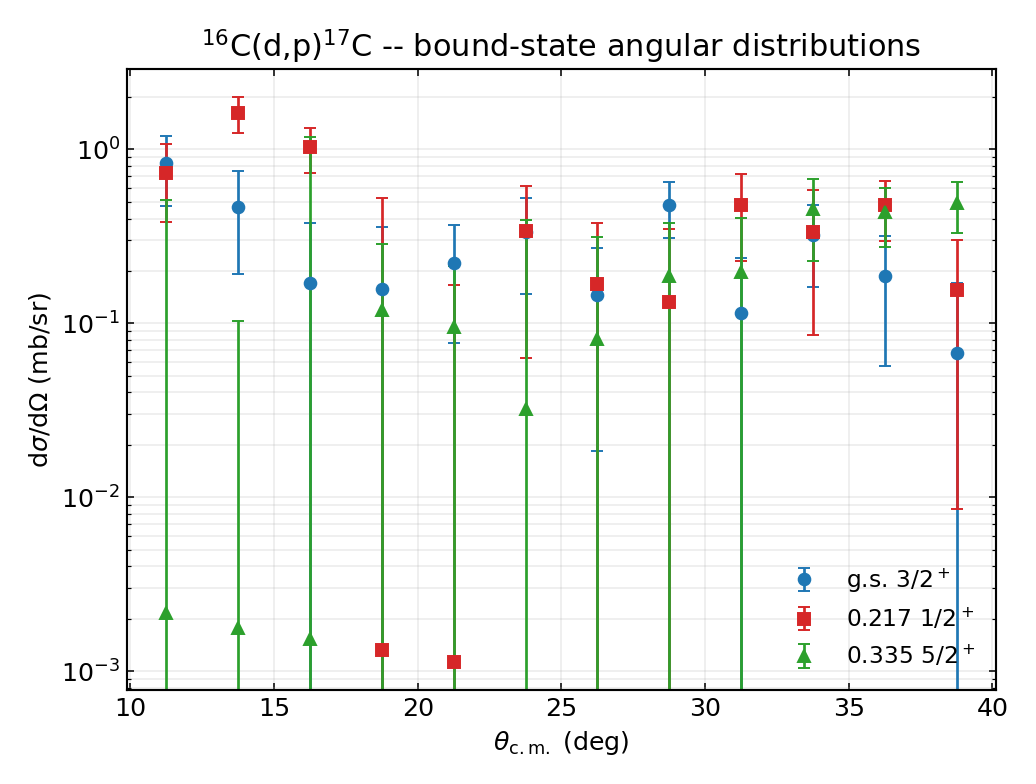
\includegraphics[width=\linewidth]{bound_states_ad.png}
    \end{column}
    \begin{column}{0.38\textwidth}
      \small
      Three bound \Cse\ states extracted as a cross-check of the machinery:
      \begin{itemize}
        \item g.s.\ $3/2^+$
        \item $0.217$ MeV $1/2^+$
        \item $0.335$ MeV $5/2^+$ (weakly populated)
      \end{itemize}
      \vspace{0.4em}
      Forward-peaked shapes consistent with the expected $\ell$ content; used to
      validate the efficiency correction and the absolute scale before turning to
      the unbound region.\\[0.4em]
      {\footnotesize $35$--$40^\circ$ bins hit the fit floor at the AT-TPC
      kinematic edge -- excluded.}
    \end{column}
  \end{columns}
\end{frame}

% ======================================================================
\section{Absolute normalization}

\begin{frame}{Absolute normalization: the idea}
  \begin{itemize}
    \item Counts $\to$ cross section uses a fixed luminosity constant:
      \[
        \frac{\mathrm{d}\sigma}{\mathrm{d}\Omega}
        = \frac{Y}{N_{\mathrm{beam}}\,N_{\mathrm{target}}\,\Delta\Omega}\cdot 10
          \;\Big/\;\varepsilon ,
      \]
      $N_{\mathrm{beam}}=1.6146\times10^{5}$, $N_{\mathrm{target}}=0.019632$,
      $\Delta\Omega = 2\pi(\cos\theta_{\mathrm{lo}}-\cos\theta_{\mathrm{hi}})$.
    \item \textbf{Cross-check:} the \Cs(d,d) elastic channel shares the entrance
      partition (same beam, D$_2$ target, luminosity). An absolute optical-model
      elastic cross section that reproduces the data \textbf{validates the constant}
      with no free normalization.
    \item Self-contained partial-wave OM solver (\texttt{om\_elastic.py}):
      Numerov $+$ Coulomb-function matching; verified vs Rutherford in the
      point-charge limit ($10^{-3}$). $E_{\mathrm{lab}}(d)=23.55$ MeV,
      $E_{\mathrm{c.m.}}=20.92$ MeV.
  \end{itemize}
\end{frame}

\begin{frame}{Absolute normalization: vertex-$z$ slicing}
  \begin{itemize}
    \item $N_{\mathrm{target}}=0.019632$ = \textbf{full-detector} D$_2$ areal
      density ($z\!\in\![0,0.99]$ m) $\approx$ per-metre. Yields from a slice
      $[z_{\rm lo},z_{\rm hi}]$ carry $1/\Delta z$, $\Delta z=z_{\rm hi}-z_{\rm lo}$ (m):
      $\dfrac{\mathrm{d}\sigma}{\mathrm{d}\Omega} = \dfrac{Y}{N_{\mathrm{beam}} N_{\mathrm{target}} \Delta\Omega}\cdot 10\,/\,\Delta z$.
    \item The divisor is the \textbf{slice thickness in m}, \emph{not} an $E_x$
      bin width:
  \end{itemize}
  \vspace{-0.3em}
  \begin{center}\small
  \begin{tabular}{ccc}
    \toprule
    vertex-$z$ slice (m) & $\Delta z$ (m) & divisor \\
    \midrule
    $[0.1,0.5]$ & 0.4 & $/0.4$ \\
    $[0.8,1.0]$ & 0.2 & $/0.2$ \\
    $\mathbf{[0.9,1.0]}$ (bound states) & \textbf{0.1} & $\mathbf{/0.1}$ \\
    \bottomrule
  \end{tabular}
  \end{center}
  \begin{itemize}
    \item Unbound analysis uses the \emph{full} range (full peak areas)
      $\Rightarrow$ no $\Delta z$ factor.
    \item \good\ \textbf{Elastic consistency:} $(d,d)$ is full-range; the
      first-principles OM match (data/OM $\approx0.86$--$0.98$) fixes
      $N_{\mathrm{beam}}N_{\mathrm{target}}$ at full thickness, and $/\Delta z$
      puts the slice on that scale to $\sim$1\% ($0.99/0.1=9.9$ vs $10$).
  \end{itemize}
\end{frame}

\begin{frame}{Absolute normalization: result}
  \begin{columns}[T]
    \begin{column}{0.6\textwidth}
      \centering
      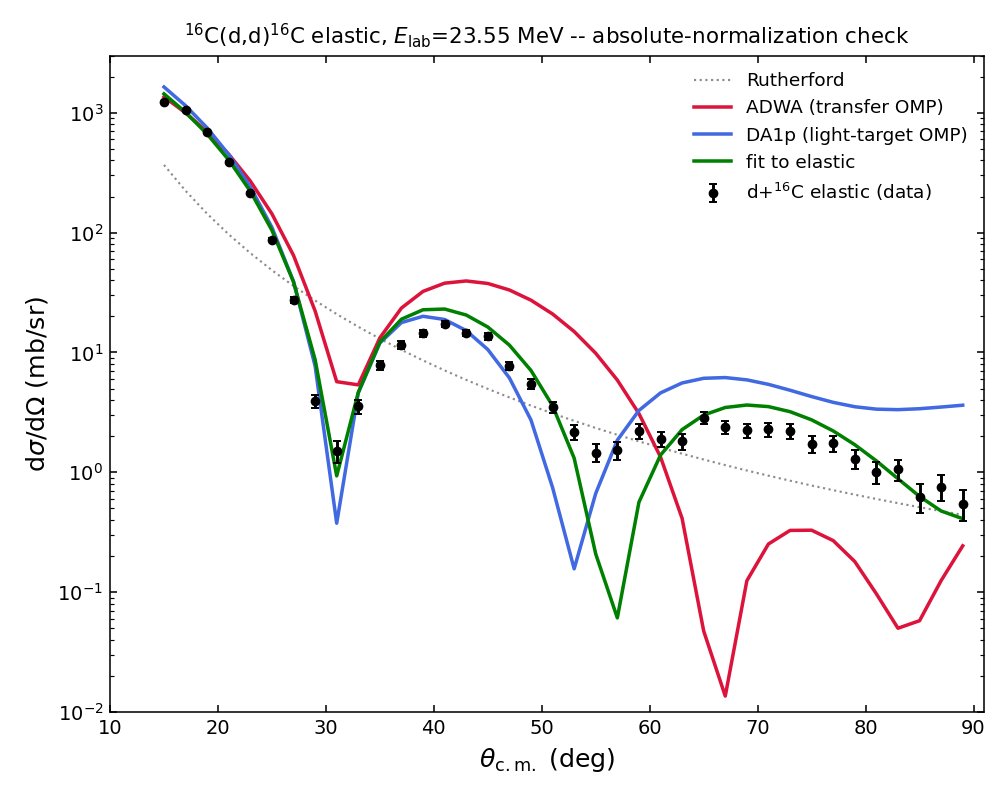
\includegraphics[width=\linewidth]{om_elastic_dd.png}
    \end{column}
    \begin{column}{0.4\textwidth}
      \small
      Forward-lobe error-weighted $\langle \mathrm{data/OM}\rangle$:
      \vspace{0.4em}
      \begin{tabular}{@{}lcc@{}}
        \toprule
        OMP & \chinu & $\langle$d/OM$\rangle$\\
        \midrule
        ADWA (transfer) & 398 & 0.864\\
        DA1p (global)   & 105 & 0.886\\
        free 5-par fit  & 32  & \textbf{0.978}\\
        \bottomrule
      \end{tabular}
      \vspace{0.6em}\\
      \good\ Absolute scale consistent with unity -- \textbf{no rescale}.\\[0.3em]
      \warn\ The transfer ADWA potential itself sits $\sim$14\% low; the honest
      figure is the \textbf{cross-potential spread $\approx$0.86--0.98 ($\sim$12\%)},
      quoted as a \emph{global} scale uncertainty (not in the per-point error).
    \end{column}
  \end{columns}
\end{frame}

\begin{frame}{From counts to \dsdo: the error model}
  \begin{block}{Per-point statistical error}
    \[
      \delta\!\left(\tfrac{\mathrm{d}\sigma}{\mathrm{d}\Omega}\right)
      = \frac{\mathrm{d}\sigma}{\mathrm{d}\Omega}\,
        \sqrt{\left(\frac{\delta Y}{Y}\right)^2 + \left(\frac{\delta\varepsilon}{\varepsilon}\right)^2}
    \]
    $\delta Y$ = Minuit amplitude error ($\chi^2$ fit to $\sqrt{N}$-weighted
    histograms $\Rightarrow$ already carries Poisson statistics).
  \end{block}
  \begin{itemize}
    \item \warn\ \textbf{Fixed (2026-05-30):} a previous
      $\sqrt{1/Y + (\delta Y/Y)^2}$ \emph{double-counted} the Poisson term
      ($\sqrt{2}$ inflation in the Poisson limit). E.g.\ g.s.\ $10$--$12.5^\circ$:
      $0.433\to0.356$ mb/sr.
    \item Three uncertainty layers: \textbf{statistical} (above) $\,+\,$
      \textbf{systematic} (82-variant envelope) $\,+\,$ \textbf{global scale}
      ($\sim$12\% from the OMP spread).
  \end{itemize}
\end{frame}

% ======================================================================
\section{Angular distributions and $L$ assignments}

\begin{frame}{Unbound resonances: \dsdo\ with systematic band}
  \centering
  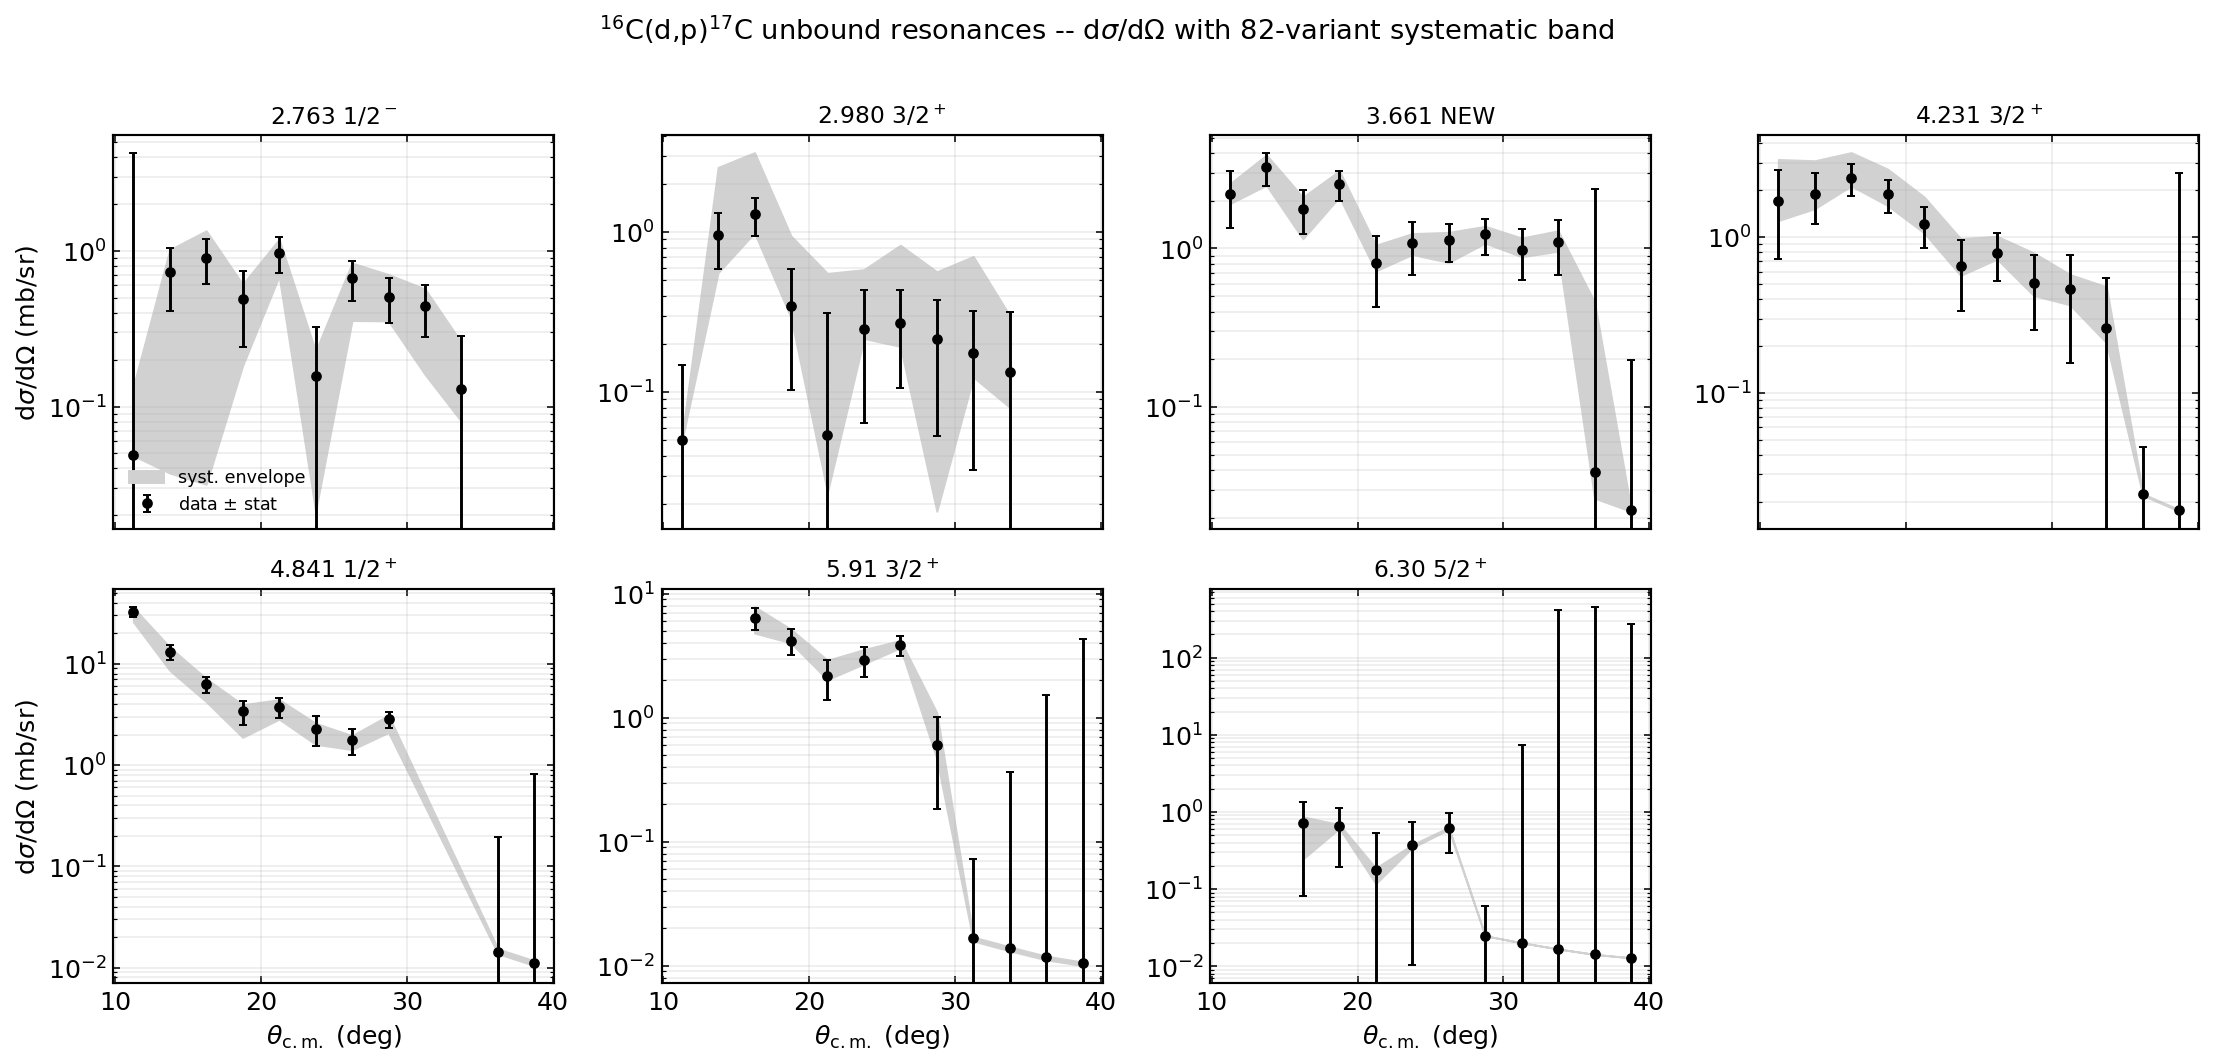
\includegraphics[width=0.96\linewidth]{unbound_ad_grid.png}\\
  {\footnotesize Black: data $\pm$ corrected statistical error. Gray band:
  min--max across the 82 spectral-fit variants. Fits use \thcm$\le30^\circ$
  (kinematic-edge bins excluded).}
\end{frame}

\begin{frame}{$L$ assignment: method}
  \begin{itemize}
    \item FRESCO 7-state DWBA with the Johnson--Soper \textbf{ADWA} effective
      deuteron OMP (sum of Koning--Delaroche $p+$\Cs\ and $n+$\Cs\ at $E_d/2$).
    \item Four templates $L=0,1,2,3$ (transferred neutron in $3s_{1/2}$,
      $2p_{1/2}$, $2d_{3/2}$/$2d_{5/2}$, $1f_{5/2}$), all in the
      \textbf{weakly-bound approximation} ($b_e=0.5$ MeV).
    \item Each extracted AD fit to each $L$ shape with a single normalization;
      best $L$ by \chinu\ on \thcm$\le30^\circ$.
    \item \textcolor{red}{Shape-only}: the WBA reproduces the $L$-dependent angular
      shape but \emph{not} the magnitude $\Rightarrow$ $C^2S$ are effective, not
      publication SFs (needs CDCC / pole-residue).
  \end{itemize}
\end{frame}

\begin{frame}{$L$ assignment: results}
  \begin{columns}[T]
    \begin{column}{0.56\textwidth}
      \centering
      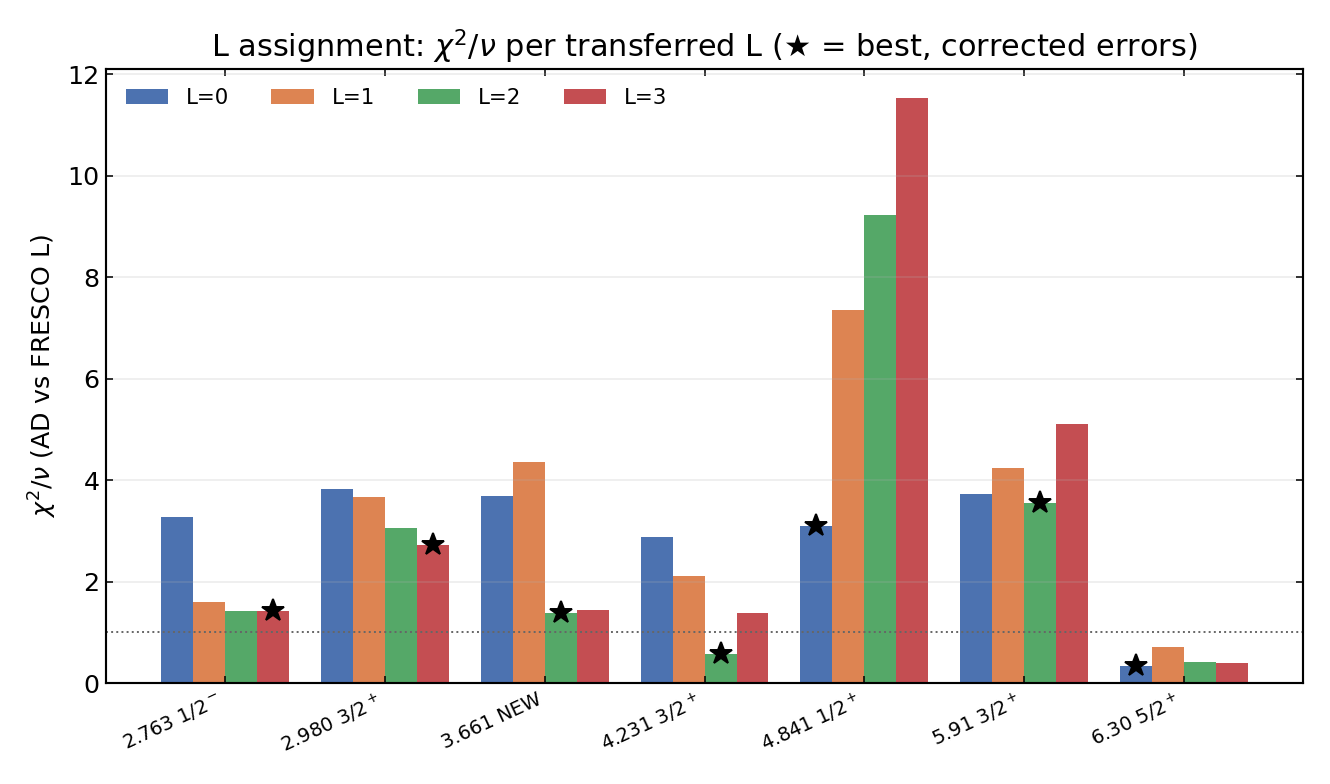
\includegraphics[width=\linewidth]{lscan_bars.png}
    \end{column}
    \begin{column}{0.44\textwidth}
      \scriptsize
      \begin{tabular}{@{}llll@{}}
        \toprule
        \Ex & lit.\ $J^\pi$ & best $L$ & next $L$\\
        \midrule
        2.763 & $1/2^-$ & $L{=}3$ (1.41) & $L{=}2$ (1.42)\\
        2.980 & $3/2^+$ & $L{=}3$ (2.73) & $L{=}2$ (3.05)\\
        3.661 & new     & \textbf{$L{=}2$ (1.38)} & $L{=}3$ (1.45)\\
        4.231 & $3/2^+$ & \textbf{$L{=}2$ (0.58)} & $L{=}3$ (1.38)\\
        4.841 & $1/2^+$ & \textbf{$L{=}0$ (3.09)} & $L{=}1$ (7.35)\\
        5.91  & $3/2^+$ & $L{=}2$ (3.55) & $L{=}0$ (3.73)\\
        6.30  & $5/2^+$ & $L{=}0$ (0.34) & $L{=}3$ (0.40)\\
        \bottomrule
      \end{tabular}
      \vspace{0.6em}\\
      \normalsize
      Numbers are \chinu\ with the \textbf{corrected} error bars
      (refreshed 2026-05-30). All best-$L$ picks and tie flags are
      \textbf{unchanged} vs the old errors; \chinu\ simply rose $\times1.3$--$1.5$.
    \end{column}
  \end{columns}
\end{frame}

\begin{frame}{$L$ assignment: state-by-state}
  \small
  \begin{itemize}
    \item \textbf{4.231 $3/2^+$ / 4.841 $1/2^+$}: decisive ($L{=}2$ $d$-wave;
      $L{=}0$ $s$-wave) -- next $L$ worse by factor $\gtrsim2$; match the PDF.
    \item \textbf{3.661 (new)}: $L{=}2$ over $L{=}3$ ($1.38$ vs $1.45$) -- not
      decisive; possible $sd$-$pf$ intruder.
    \item \textbf{2.763 $1/2^-$}: three-way near-tie ($L{=}3/2/1$); AD too flat to
      separate.
    \item \textbf{2.980 $3/2^+$}: \warn\ no template fits well; $17.5^\circ$ AD peak
      not reproduced; spectral fit wants $E_0\sim120$ keV above the SM prior.
    \item \textbf{6.30 $5/2^+$}: $L{=}0$ has best \chinu\ but is \emph{forbidden}
      ($0^+\!\otimes s_{1/2}=1/2^+$); the physically allowed $L{=}2/3$ are tied.
    \item \textbf{5.91 $3/2^+$}: $L{=}2$ marginal over $L{=}0$; AD poorly
      constrained past $30^\circ$.
  \end{itemize}
\end{frame}

% ======================================================================
\section{Systematics and summary}

\begin{frame}{Systematic envelope (82 variants)}
  \begin{columns}[T]
    \begin{column}{0.6\textwidth}
      \centering
      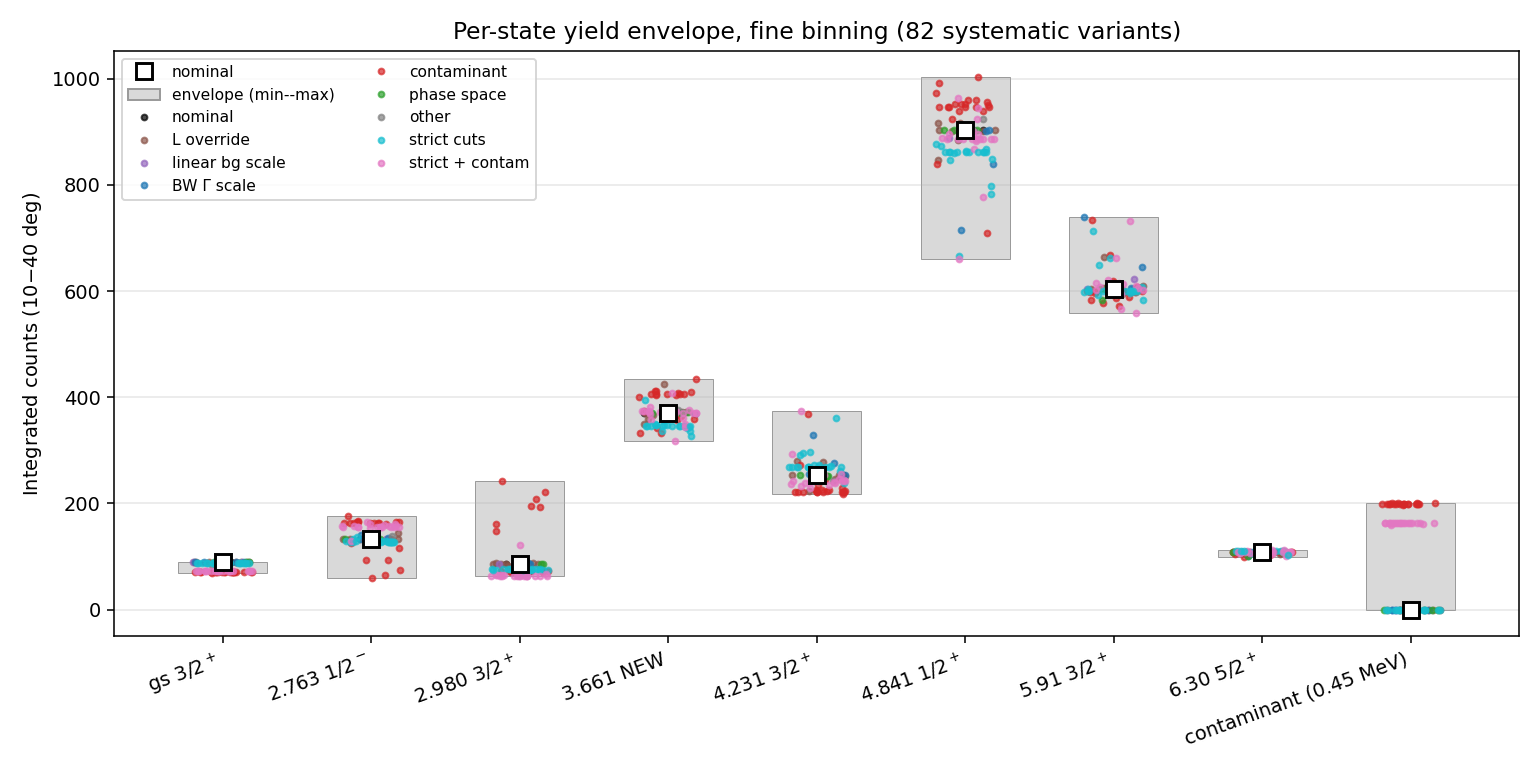
\includegraphics[width=\linewidth]{yield_envelope_fine.png}
    \end{column}
    \begin{column}{0.4\textwidth}
      \scriptsize
      Per-state integrated-yield envelope (min--max across variants):
      \vspace{0.3em}
      \begin{tabular}{@{}lcc@{}}
        \toprule
        state & $-\%$ & $+\%$\\
        \midrule
        g.s.\ $3/2^+$ & $-23$ & $+0$\\
        2.763 & $-56$ & $+32$\\
        2.980 & $-28$ & $+179$\\
        3.661 & $-15$ & $+17$\\
        4.231 & $-14$ & $+48$\\
        4.841 & $-27$ & $+11$\\
        5.91  & $-8$  & $+22$\\
        6.30  & $-9$  & $+3$\\
        \bottomrule
      \end{tabular}
      \vspace{0.4em}\\
      \normalsize
      Largest model-dependence: \textbf{2.763 \& 2.980} (contaminant
      degeneracy). \textbf{6.30} robust.
    \end{column}
  \end{columns}
\end{frame}

\begin{frame}{Summary}
  \begin{itemize}
    \item Per-state absolute \dsdo\ extracted for the 3 bound and 7 unbound
      \Cse\ states from \Cs\dpr\ at 11.77 MeV/u.
    \item \good\ \textbf{Absolute scale validated} against \Cs(d,d) elastic; the
      normalization uncertainty is the $\sim$12\% OMP spread (global).
    \item \good\ \textbf{Error model corrected}: per-point statistics no longer
      double-counted; statistical $+$ systematic $+$ scale layers separated.
    \item \good\ \textbf{$L$ assignments} robust to the error fix:
      4.231 ($L{=}2$) and 4.841 ($L{=}0$) decisive; 3.661, 2.763, 5.91 ambiguous;
      2.980 and 6.30 problematic (shape / selection-rule).
    \item \textbf{Deliverable} (this repo): yields, \dsdo, and the systematic
      envelope. Final $L$ / $C^2S$ done downstream by the theorist with a
      CDCC-grade treatment.
  \end{itemize}
\end{frame}

\begin{frame}{Open items}
  \begin{itemize}
    \item Fold the $\sim$12\% elastic-normalization scale into the published
      \dsdo / yield bands (common multiplicative factor).
    \item Continuum-form tests (quadratic/exp bg, PS-shape variation) to show the
      $0.45$ MeV contaminant is not bg flexibility.
    \item Physically identify the $0.45$ MeV excess ($vertex_z$, $\theta_{\rm lab}$
      fingerprint of a non-D$_2$ channel?).
    \item CDCC / pole-residue treatment for publication-grade absolute $C^2S$.
  \end{itemize}
  \vspace{1em}
  \centering
  \footnotesize Refs: Pereira-Lopez \textit{et al.}, PLB 811 (2020) 135939;
  Movilla \& Ayyad (2026). Pang \textit{et al.}, arXiv:1606.01507 (DA1p OMP).
\end{frame}

\end{document}
